\documentclass[xcolor={usenames,svgnames,x11names,table}]{beamer}

\usetheme{SBU}

\hypersetup{pdfstartview={Fit}}

\usepackage{mypackages}
\usepackage{mycommands}
\usepackage{multimedia}
\usepackage{adjustbox}
%%%%%%%%%%TIKZ
\usetikzlibrary{positioning,shapes,shadows,arrows}

\tikzstyle{abstract}=[rectangle, draw=RoyalBlue, thick, rounded corners, fill=white, drop shadow,
        text centered, anchor=north, text=black, text width=3cm]
\tikzstyle{comment}=[rectangle, draw=black, rounded corners, fill=green, drop shadow,
        text centered, anchor=north, text=white, text width=3cm]
\tikzstyle{myarrow}=[->, >= triangle 90, thick]
\tikzstyle{line}=[-, thick]
%%%%%%%%%%%
\usetikzlibrary{backgrounds}

\title[A Game of Tiers]{%
    \texorpdfstring{%
    A Game of Tiers: \\ Exploring the Formal Properties of \\ TSL Languages}
    {A Game of Tiers: \\ Exploring the Formal Properties of TSL Languages}
    }
\author[DeSanto]{\texorpdfstring{%
                            Aniello De Santo
                            }
                            {Aniello De Santo} 
                        }
%\institute{Department of Linguistics \\ Stony Brook University\\\texttt{aniello.desanto@stonybrook.edu}}
\date{Computational Phonology Workshop\\Dec 12, 2016}


\begin{document}
\unnumbered{
\begin{frame}[plain]
\begin{center}
\includegraphics[scale=0.4]{img/lingo-logo.png}
\end{center}
\vspace{-0.5cm}
	\titlepage
\end{frame}
}


%=====================OVERVIEW================%
\unnumbered{

\begin{frame}{The Talk in a Nutshell}
	\begin{block}{Subregular Hypothesis  for Phonology}
		\begin{itemize}
		\item Phonotactic patterns can be described by classes in the subregular hierarchy;
		\item Pin-pointing the right class will be useful for  typology, learnability, cognitive predictions ...
		\end{itemize}
	\end{block}

	\pause

	\begin{alertblock}{Current Hypothesis}
		\begin{itemize}
		\item Tier-based Strictly Local seems to be the right fit;
		\item  But ... several problematic patterns have been reported!
		\end{itemize}
	\end{alertblock}

	\pause

	\begin{block}{Idea}
		We can explore (minimal) extensions to TSL
	\end{block}

\end{frame}

\begin{frame}{Outline}
   \tableofcontents
\end{frame}
}

%===============================PRELIMINARIES=============================%
\section[Preliminaries]{Preliminaries}

\begin{frame}{Phonology as a Subregular System}


	\begin{columns}
	\column{.40\linewidth}
	%SUBREGULAR REGION
	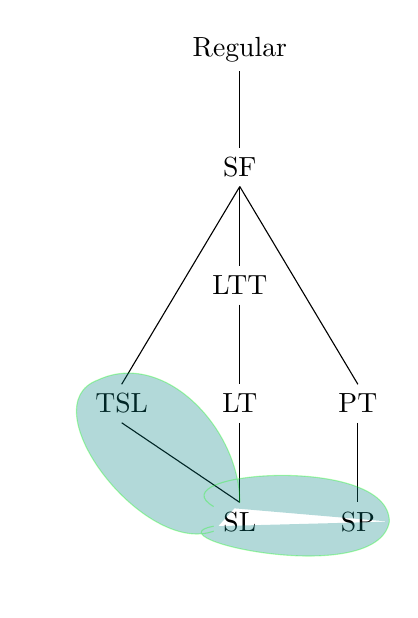
\begin{tikzpicture}[ 
   	 highlight/.style = { draw, rectangle, dashed }
    	]
        \node (R) at (0,10) {Regular};
        \node (SF) at (0,8.5) {SF};
        \node (LTT) at (0,7) {LTT};
        \node (LT) at (0,5.5) {LT};
        \node (SL) at (0,4) {SL};
        %
        \node (PT) at (1.5,5.5) {PT};
        \node (SP) at (1.5,4) {SP};
        %
        \node (TSL) at (-1.5,5.5) {TSL};
        %
        \foreach \Source/\Target in {%
                R.south/SF.north,
                SF.south/LTT.north,
                LTT.south/LT.north,
                LT.south/SL.north,
                SF.south/PT.north,
                PT.south/SP.north,
                SF.south/TSL.north,
                TSL.south/SL.north%
            }
        \draw (\Source) to (\Target);
        
        \visible<2->{ \draw[green, fill=teal, opacity=0.3] (1.9,4)%
        	to [out=260, in=190] (SL)%
        	to [out=200, in=200] (-1.8,5.8)%260-230
        	to [out=25, in=90] (SL)%
        	to [out=150, in=90] (1.9,4);}
        %
        %
        
        \end{tikzpicture}
            
    
    \column{.5\linewidth}
   	 \begin{block}{Subregular Hypothesis}
    		\begin{itemize}
    		\item Phonology is  \textbf{\textcolor{teal!75}{subregular}};
    		\item Local phonotactic dependencies are Strictly Local.
    		\end{itemize}
    	\end{block}

	\onslide<3->{
	\begin{exampleblock}{SL: Example}
		Word-final devoicing: $^* [+\textit{voice}]\ltimes$

		\begin{center}
		\begin{tikzpicture} %%%%%DEVOICING IN GERMAN

		\node (1) at (0.5,0) {$\rtimes$ };
		\node (2) at (1,0) {r};
		\node (3) at (1.5,0) {a};
		\node (4) at (2,0.05) {d};
		\node (5) at (2.5,0) {$\ltimes$};
		
		\visible<4->{\draw [dashed, red] (1.7, -0.2) -- (2.7, -0.2) -- (2.7,0.3) -- (1.7,0.3) -- (1.7, -0.2);
		\node (00) at (-0.15,0.1) {$^*$};}


		\begin{scope}[yshift=-30pt]
		\node (1) at (0.5,0) {$\rtimes$ };
		\node (2) at (1,0) {r};
		\node (3) at (1.5,0) {a};
		\node (4) at (2,0.05) {t};
		\node (5) at (2.5,0) {$\ltimes$};

		\visible<5->{\draw [dashed, DarkGreen] (1.7, -0.2) -- (2.7, -0.2) -- (2.7,0.3) -- (1.7,0.3) -- (1.7, -0.2);
		\node (00) at (-0.15,0.1) {$^{ok}$};}
		\end{scope}

		\end{tikzpicture}
		\end{center}
	\end{exampleblock}
		}
%
	\end{columns}
	\centering
	\vspace{0.3cm}
	\onslide<4->{\alert{What about unbounded dependencies?}}
\end{frame}

\begin{frame}{Long Distance Dependencies as Tier-based Strictly Local}

    \begin{itemize}
    \item Problem: Unbounded processes cannot be captured by Strictly Local Grammars
    \item Solution: Select a subset of segments and enforce constraints only over it.
    \end{itemize}
    
    \begin{block}{Tier-based Strictly Local  (TSL) Grammars}
    	\begin{itemize}
    		\item a projection function $E: \Sigma \rightarrow T$ with $T \subseteq \Sigma$\\
    	$\Rightarrow$ projection on a tier is determined just by the "shape" of the segment (no structural or "proximity" information);
    		\item strictly local constraints over T;
    	\end{itemize}
    \end{block}
\end{frame}
    
\begin{frame}{TSL Example: Sibilant harmony in \textsc{Aari}}

    \begin{exampleblock}{Grammar}
    T = \{s, z,  \textctyogh,  \textesh  \} 
    S = \{$^*$\textctyogh s, $^*$s\textctyogh, $^*$s\textesh, $^*$\textesh s  \}
    \end{exampleblock}
    \begin{center}
    
    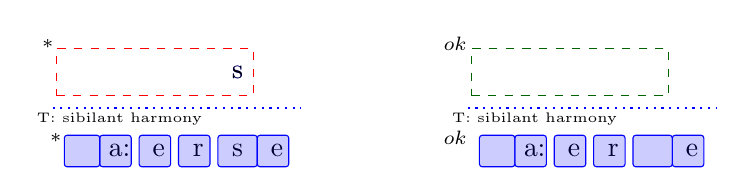
\begin{tikzpicture} % AARI TIERS EXAMPLE
    
    \node (00) at (-0.3,0.1) {$^*$};
    \node (0) at (0,0) {\textctyogh };
    \node (1) at (0.5,0) {a:};
    \node (2) at (1,0) {e};
    \node (3) at (1.5,0) {r};
    \node (4) at (2,0) {s};
    \node (5) at (2.5,0) {e};
    %tier
     \visible<2->{\draw[dotted, thick, blue] (-0.35,0.55) to (2.8,0.55);
    \node at (0.5,0.40) {{\tiny T: sibilant harmony}};
    }
    \visible<8->{\node (000) at (-0.4,1.3) {$^*$};}
    \visible<2>{\node[blue] (00) at (0,1) {\textctyogh };}
    \visible<3->{\node (00) at (0,1) {\textctyogh };}
    \visible<6>{\node[blue] (05) at (2,1) {s};}
    \visible<7->{\node (05) at (2,1) {s};}
    %projection function
    \visible<2>{\filldraw [blue, rounded corners=1, fill opacity=.2,draw opacity=1] (-0.2,-0.2 ) rectangle (0.25, 0.2);}
    \visible<3>{\filldraw [blue, rounded corners=1, fill opacity=.2,draw opacity=1] (0.25,-0.2 ) rectangle (0.65, 0.2);}
    \visible<4>{\filldraw [blue, rounded corners=1, fill opacity=.2,draw opacity=1] (0.75,-0.2 ) rectangle (1.15, 0.2);}
    \visible<5>{\filldraw [blue, rounded corners=1, fill opacity=.2,draw opacity=1] (1.25,-0.2 ) rectangle (1.65, 0.2);}
    \visible<6>{\filldraw [blue, rounded corners=1, fill opacity=.2,draw opacity=1] (1.75,-0.2 ) rectangle (2.25, 0.2);}
    \visible<7>{\filldraw [blue, rounded corners=1, fill opacity=.2,draw opacity=1] (2.25,-0.2 ) rectangle (2.65, 0.2);}
   %local contraints 
    \visible<8->{\draw [dashed, red] (-0.3, 0.7) -- (2.2, 0.7) -- (2.2,1.3) -- (-0.3,1.3) -- (-0.3, 0.7);}

    \begin{scope}[xshift=150pt] %right example
    
    \node (0) at (0,0) {\textctyogh };
    \node (1) at (0.5,0) {a:};
    \node (2) at (1,0) {e};
    \node (3) at (1.5,0) {r};
    \node (4) at (2,0) {\textesh };
    \node (5) at (2.5,0) {e};
    \node (00) at (-0.5,0.1) {$^{ok}$};
    %tier
    \visible<16->{\node (000) at (-0.5,1.3) {$^{ok}$};}
    \visible<10>{\node[blue] (00) at (0,1) {\textctyogh };}
    \visible<11->{\node (00) at (0,1) {\textctyogh };}
    \visible<14>{\node[blue] (05) at (2,1) {\textesh };}
    \visible<15->{\node (05) at (2,1) {\textesh };}
    %projection function
    \visible<10>{\filldraw [blue, rounded corners=1, fill opacity=.2,draw opacity=1] (-0.2,-0.2 ) rectangle (0.25, 0.2);}
    \visible<11>{\filldraw [blue, rounded corners=1, fill opacity=.2,draw opacity=1] (0.25,-0.2 ) rectangle (0.65, 0.2);}
    \visible<12>{\filldraw [blue, rounded corners=1, fill opacity=.2,draw opacity=1] (0.75,-0.2 ) rectangle (1.15, 0.2);}
    \visible<13>{\filldraw [blue, rounded corners=1, fill opacity=.2,draw opacity=1] (1.25,-0.2 ) rectangle (1.65, 0.2);}
    \visible<14>{\filldraw [blue, rounded corners=1, fill opacity=.2,draw opacity=1] (1.75,-0.2 ) rectangle (2.25, 0.2);}
    \visible<15>{\filldraw [blue, rounded corners=1, fill opacity=.2,draw opacity=1] (2.25,-0.2 ) rectangle (2.65, 0.2);}
    %local constraints
    \visible<16->{\draw [dashed, DarkGreen] (-0.3, 0.7) -- (2.2, 0.7) -- (2.2,1.3) -- (-0.3,1.3) -- (-0.3, 0.7);}
    %tier level
    \visible<9->{
    \draw[dotted, thick, blue] (-0.35,0.55) to (2.8,0.55);
    \node at (0.5,0.40) {{\tiny T: sibilant harmony}};
    }
    
    \end{scope}
    
    \end{tikzpicture}
    \end{center} 
\end{frame}

        
%========================TSL LIMITS ==================%
\section[TSL Limits]{TSL Limits}      
 
\begin{frame}{Problematic Patterns (1/2)}

	\begin{block}{Sibilant Harmony in \textsc{Imdlawn Tashlhiyt} \textbf{(McMullin2016)}}
	\vspace{-0.3cm}
	
	\begin{table}[h!] % DATA

        \begin{tabular}{llll}
        \multicolumn{4}{l}{1) Underlying causative prefix /s(\textlengthmark)-/} \\
               & \emph{Base}       &  \emph{Causative}     &                                   \\
        a.     & uga        & \ExampleT{s}\textlengthmark-uga         & "be evacuated"                    \\
        b.     & a\ExampleT{s}\textlengthmark twa     &  \ExampleT{s}-a\ExampleT{s}\textlengthmark twa      & "settle, be levelled"             \\
        \\ \vspace{-0.6cm} \\
        \multicolumn{4}{l}{\onslide<2->{  2) Sibilant harmony}}                 \\
        \onslide<2->{       & \emph{Base}        &  \emph{Causative}     &                                   \\
        a.     & fia\ExampleT{\textipa{S}}r     & \ExampleT{\textipa{S}}- fia\ExampleT{\textipa{S}}r     & "be full of straw, of discord"    \\
        b.     & n\ExampleT{z}a        &\ExampleT{z}\textlengthmark-n\ExampleT{z}a        & "be sold"   \\}
        \\ \vspace{-0.6cm} \\
        \multicolumn{4}{l}{\onslide<3->{ 3) Sibilant voicing harmony blocked}} \\
        \onslide<3->{        & \emph{Base}       &  \emph{Causative}     &                                   \\
        a.     & u\alert{k}\ExampleT{z}        & \ExampleT{s}\textlengthmark-u\alert{k}\ExampleT{z}      & "recognize"                    \\
        b.     &  \alert{q}\textlengthmark u\ExampleT{\textyogh}\textlengthmark i     &  \ExampleT{\textipa{S}}- \alert{q}u\ExampleT{\textyogh}\textlengthmark i    & "be dislocated, broken"      }
                        
        \end{tabular}
        \end{table}

	\vspace{-0.3cm}
	\end{block}

	\centering
	\onslide<4->{    \alert{Can we write a TSL grammar to capture this pattern?}}
\end{frame}   
 
\begin{frame}{ Sibilant Harmony in \textsc{Imdlawn Tashlhiyt}  }%MCMULLIN Imdlawn Tashlhiyt TIER EXAMPLES

        \begin{block}{Generalization (1/2)}
        		Sibilants must agree in anteriority and voicing.
        \end{block}
         
         \begin{exampleblock}{Grammar}
          $T = \{$ \textit{\textctyogh}, s, z,\textit{\textesh}$ \}$  \\
          $S= \{$ $^*$s\textctyogh, $^*$sz, $^*$s\textesh, $^*$\textctyogh s,$^*$\textesh s,  $^*$zs, $^*$z\textesh,  $^*$z\textctyogh, $^*$\textesh z, $^*$\textesh  \textctyogh, $^*$\textctyogh \textesh, $^*$\textctyogh z $\}$
          \end{exampleblock}
         

        \begin{center}
        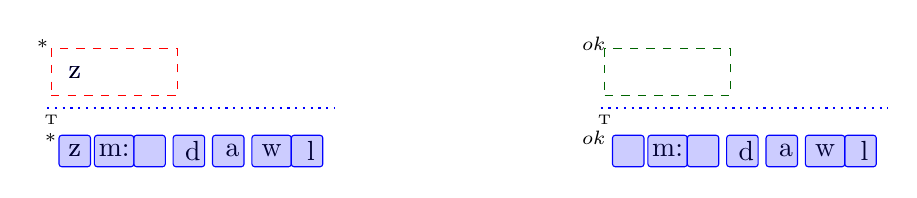
\begin{tikzpicture} % Imdlawn Tashlhiyt TIER EXAMPLES
        \node (000) at (-0.8,0.1) {$^*$};
        \node (00) at (-0.5,0) {z};
        \node (00) at (-0.5,0) {z};
        \node (0) at (0,0) {m:};
        \node (1) at (0.5,0) {\textctyogh };
        \node (2) at (1,0) {d};
        \node (3) at (1.5,0) {a};
        \node (4) at (2,0) {w};
        \node (5) at (2.5,0) {l};
        %tier level
        \visible<2->{
        \draw[dotted, thick, blue] (-0.85,0.55) to (2.8,0.55);
        \node at (-0.8,0.40) {{\tiny T}};
        }
        
        \visible<2>{\node[blue] (00') at (-0.5,1) {z};}
        \visible<3->{\node (00') at (-0.5,1) {z};}
        \visible<4>{\node[blue] (1) at (0.5,1) {\textctyogh };}
        \visible<5->{\node (1) at (0.5,1) {\textctyogh };}
	%local constraints on tier
        \visible<9->{
        \node (000) at (-0.9,1.3) {$^*$};
        \draw [dashed, red] (-0.8, 0.7) -- (0.8, 0.7) -- (0.8,1.3) -- (-0.8,1.3) -- (-0.8, 0.7);
        }
        %projection  function
        \visible<2>{\filldraw [blue, rounded corners=1, fill opacity=.2,draw opacity=1] (-0.7,-0.2 ) rectangle (-0.3, 0.2);}
        \visible<3>{\filldraw [blue, rounded corners=1, fill opacity=.2,draw opacity=1] (-0.25,-0.2 ) rectangle (0.25, 0.2);}
        \visible<4>{\filldraw [blue, rounded corners=1, fill opacity=.2,draw opacity=1] (0.25,-0.2 ) rectangle (0.65, 0.2);}
        \visible<5>{\filldraw [blue, rounded corners=1, fill opacity=.2,draw opacity=1] (0.75,-0.2 ) rectangle (1.15, 0.2);}
        \visible<6>{\filldraw [blue, rounded corners=1, fill opacity=.2,draw opacity=1] (1.25,-0.2 ) rectangle (1.65, 0.2);}
        \visible<7>{\filldraw [blue, rounded corners=1, fill opacity=.2,draw opacity=1] (1.75,-0.2 ) rectangle (2.25, 0.2);}
        \visible<8>{\filldraw [blue, rounded corners=1, fill opacity=.2,draw opacity=1] (2.25,-0.2 ) rectangle (2.65, 0.2);}
        
        \begin{scope}[xshift=200pt] %example on the right

        \node (000) at (-0.93,0.1) {$^{ok}$};
        \node (00) at (-0.5,0) {\textctyogh};
        \node (0) at (0,0) {m:};
        \node (1) at (0.5,0) {\textctyogh };
        \node (2) at (1,0) {d};
        \node (3) at (1.5,0) {a};
        \node (4) at (2,0) {w};
        \node (5) at (2.5,0) {l};
 
        %tier
        \visible<10->{
        \draw[dotted, thick, blue] (-0.85,0.55) to (2.8,0.55);
        \node at (-0.8,0.40) {{\tiny T}};
        }
        \visible<10>{\node[blue] (00') at (-0.5,1) {\textctyogh};}
        \visible<11->{\node (00') at (-0.5,1) {\textctyogh};}
        \visible<13>{\node[blue] (1) at (0.5,1) {\textctyogh };}
        \visible<14->{\node (1) at (0.5,1) {\textctyogh };}
        %projection function
        \visible<10>{\filldraw [blue, rounded corners=1, fill opacity=.2,draw opacity=1] (-0.7,-0.2 ) rectangle (-0.3, 0.2);}
        \visible<11>{\filldraw [blue, rounded corners=1, fill opacity=.2,draw opacity=1] (-0.25,-0.2 ) rectangle (0.25, 0.2);}
        \visible<12>{\filldraw [blue, rounded corners=1, fill opacity=.2,draw opacity=1] (0.25,-0.2 ) rectangle (0.65, 0.2);}
        \visible<13>{\filldraw [blue, rounded corners=1, fill opacity=.2,draw opacity=1] (0.75,-0.2 ) rectangle (1.15, 0.2);}
        \visible<14>{\filldraw [blue, rounded corners=1, fill opacity=.2,draw opacity=1] (1.25,-0.2 ) rectangle (1.65, 0.2);}
        \visible<15>{\filldraw [blue, rounded corners=1, fill opacity=.2,draw opacity=1] (1.75,-0.2 ) rectangle (2.25, 0.2);}
        \visible<16>{\filldraw [blue, rounded corners=1, fill opacity=.2,draw opacity=1] (2.25,-0.2 ) rectangle (2.65, 0.2);}
        %local constraints
        \visible<17->{
        \node (000) at (-0.93,1.3) {$^{ok}$};
        \draw [dashed, DarkGreen] (-0.8, 0.7) -- (0.8, 0.7) -- (0.8,1.3) -- (-0.8,1.3) -- (-0.8, 0.7);
        }
        \end{scope}
        \end{tikzpicture}
        \end{center} 
\end{frame}  

\begin{frame}{ Sibilant Harmony in \textsc{Imdlawn Tashlhiyt}} %MCMullin Imdlawn Tashlhiyt Tier example continued
         
         \begin{block}{Generalization (2/2)}
         Voiceless obstruents block agreement in voicing.
         \end{block}
         
         \begin{exampleblock}{Grammar}
          $T = \{$ \textit{\textctyogh}, s, z,\textit{\textesh}, q$ \}$  \\
          $S= \{$ $^*$s\textctyogh, $^*$sz, $^*$s\textesh, $^*$\textctyogh s,$^*$\textesh s,  $^*$zs, $^*$z\textesh,  $^*$z\textctyogh, $^*$\textesh z, $^*$\textesh  \textctyogh, $^*$ \textctyogh \textesh, $^*$\textctyogh z $\}$
         
          \end{exampleblock}
        
        
        \begin{center}
        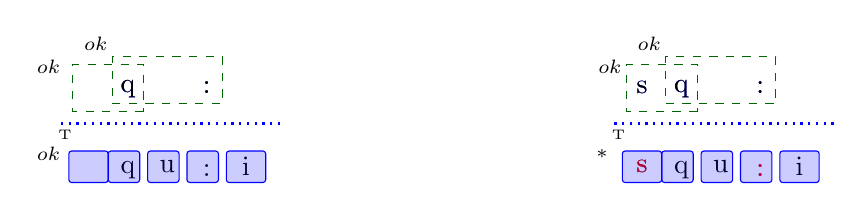
\begin{tikzpicture}%Imdlawn Tashlhiyt Tier example 
        
        \node (000) at (-0.5,0.1) {$^{ok}$};
        \node (0) at (0,0) {\textesh};
        \node (1) at (0.5,-0.05) {q};
        \node (2) at (1,0) {u};
        \node (3) at (1.5,-0.05) { \textctyogh:};
        \node (4) at (2,0) {i};
        %tier level segments
        \visible<2>{\node[blue] (01) at (0,1) {\textesh};}
        \visible<3->{\node (01) at (0,1) {\textesh};}
        \visible<3>{\node[blue] (03) at (0.5,0.98) {q};}
        \visible<4->{\node (03) at (0.5,0.98) {q};}
        \visible<5>{\node[blue] (03) at (1.5,1) { \textctyogh:};}
        \visible<6->{\node (03) at (1.5,1) { \textctyogh:};}
        %tier level
        \visible<2->{
        \draw[dotted, thick, blue] (-0.35,0.55) to (2.5,0.55);
        \node at (-0.3,0.40) {{\tiny T}};
        }
        %local constraints
        \visible<7->{
        \node (00) at (-0.5,1.2) {$^{ok}$};
        \draw [dashed, DarkGreen] (0.7, 0.7) -- (-0.2, 0.7) -- (-0.2,1.3) -- (0.7,1.3) -- (0.7, 0.7);
        }
        \visible<8->{
        \node (0000) at (0.1,1.5) {$^{ok}$};
        \draw [dashed, DarkGreen] (0.3, 0.8) -- (1.7, 0.8) -- (1.7,1.4) -- (0.3,1.4) -- (0.3, 0.8);
        }
        %projection function
        \visible<2>{\filldraw [blue, rounded corners=1, fill opacity=.2,draw opacity=1] (-0.25,-0.2 ) rectangle (0.25, 0.2);}
        \visible<3>{\filldraw [blue, rounded corners=1, fill opacity=.2,draw opacity=1] (0.25,-0.2 ) rectangle (0.65, 0.2);}
        \visible<4>{\filldraw [blue, rounded corners=1, fill opacity=.2,draw opacity=1] (0.75,-0.2 ) rectangle (1.15, 0.2);}
        \visible<5>{\filldraw [blue, rounded corners=1, fill opacity=.2,draw opacity=1] (1.25,-0.2 ) rectangle (1.65, 0.2);}
        \visible<6>{\filldraw [blue, rounded corners=1, fill opacity=.2,draw opacity=1] (1.75,-0.2 ) rectangle (2.25, 0.2);}
        
       
        \begin{scope}[xshift=200pt]%illformed one
        \node (000) at (-0.5,0.1) {$^{*}$};
        \node (0) at (0,0) {s};
        \visible<16->{\node[red] (0) at (0,0) {s};}
        \node (1) at (0.5,-0.05) {q};
        \node (2) at (1,0) {u};
        \node (3) at (1.5,-0.05) { \textctyogh:};
        \visible<16->{\node[red] (3) at (1.5,-0.05) { \textctyogh:};}
        \node (4) at (2,0) {i};
        
        %tier level nodes
        \visible<9>{\node[blue] (01) at (0,1) {s};}
        \visible<10->{\node (01) at (0,1) {s};}
        \visible<10>{\node[blue] (03) at (0.5,0.98) {q};}
        \visible<11->{\node (03) at (0.5,0.98) {q};}
        \visible<12>{\node[blue] (03) at (1.5,1) { \textctyogh:};}
        \visible<13->{\node (03) at (1.5,1) { \textctyogh:};}
        
        %tier level
        \visible<9->{
        \draw[dotted, thick, blue] (-0.35,0.55) to (2.5,0.55);
        \node at (-0.3,0.40) {{\tiny T}};
        }
        %lcoal constraints
        \visible<14->{
        \node (00) at (-0.4,1.2) {$^{ok}$};
        \draw [dashed, DarkGreen] (0.7, 0.7) -- (-0.2, 0.7) -- (-0.2,1.3) -- (0.7,1.3) -- (0.7, 0.7);
        }
        \visible<15->{
        \node (0000) at (0.1,1.5) {$^{ok}$};
        \draw [dashed, DarkGreen] (0.3, 0.8) -- (1.7, 0.8) -- (1.7,1.4) -- (0.3,1.4) -- (0.3, 0.8);
        }
        %projection function
        \visible<9>{\filldraw [blue, rounded corners=1, fill opacity=.2,draw opacity=1] (-0.25,-0.2 ) rectangle (0.25, 0.2);}
        \visible<10>{\filldraw [blue, rounded corners=1, fill opacity=.2,draw opacity=1] (0.25,-0.2 ) rectangle (0.65, 0.2);}
        \visible<11>{\filldraw [blue, rounded corners=1, fill opacity=.2,draw opacity=1] (0.75,-0.2 ) rectangle (1.15, 0.2);}
        \visible<12>{\filldraw [blue, rounded corners=1, fill opacity=.2,draw opacity=1] (1.25,-0.2 ) rectangle (1.65, 0.2);}
        \visible<13>{\filldraw [blue, rounded corners=1, fill opacity=.2,draw opacity=1] (1.75,-0.2 ) rectangle (2.25, 0.2);}
        
        \end{scope}
        \end{tikzpicture}
        \end{center} 
        
        \visible<17->{
        \centering
        \alert{No TSL grammar can block voicing and enforce anteriority!}
        }
\end{frame}  

%%%%%%%%%%%%%%%%%%%%%%%%%%%%%%%%%%%%%%%%%
%==============================SAMALA1======================%
%%%%%%%%%%%%%%%%%%%%%%%%%%%%%%%%%%%%%%%%%

\begin{frame}{Problematic Patterns (2/2)}
    \begin{block}{Sibilant Harmony in \textsc{Samala}  \textbf{(McMullin2016)} } % \cite{McMullin2016}
     \vspace{-0.6cm} 

    \begin{table}[h!] %data from McMullin
    \begin{tabular}{llll}
    \multicolumn{4}{l}{1) Unbounded sibilant harmony} \\
    \\ \vspace{-0.7cm} \\
    a.    /k-\ExampleT{s}u-\ExampleT{\textipa{S}}ojin/&  k\ExampleT{\textipa{S}}u\ExampleT{\textipa{S}}ojin  & "I darken it"  &    \\
    b.    /k-\ExampleT{s}u-k'ili-mekeken-\ExampleT{\textipa{S}}/ &  k\ExampleT{\textipa{S}}uk'ilimekeket\ExampleT{\textipa{S}}  & "I straighten up"  & \pause    \\           
    \\ \vspace{-0.6cm} \\
    \multicolumn{4}{l}{ 2)  /s/$\rightarrow$ [\textipa{S}] when preceding (adjacent) [t, n, l]}\\
    \\ \vspace{-0.7cm} \\ 
    a.   /\ExampleT{s}-\alert{l}ok'in/  & \ExampleT{\textipa{S}}\alert{l}ok'in    &  he cuts it   &  \\
    b.    /\ExampleT{s}-\alert{t}epu\textglotstop/ & \ExampleT{\textipa{S}}\alert{t}epu\textglotstop &  "he gambles"   &     \pause      \\
    \\ \vspace{-0.6cm} \\
    \multicolumn{4}{l}{ 3) Long-distance agreement overrides local disagreement}\\
    \\ \vspace{-0.7cm} \\
    a.   /\ExampleT{s}-i\ExampleT{\textipa{S}}\alert{t}-ti\ExampleT{\textipa{S}}\alert{t}i-jep-u\ExampleT{s}/  & \ExampleT{s}i\ExampleT{s}\alert{t}i\ExampleT{s}\alert{t}ijepu\ExampleT{s}   & "they show him"    &   \\
    b.   /\ExampleT{s}-\alert{n}et-u\ExampleT{s}/  &  \ExampleT{s}\alert{n}etu\ExampleT{s}  &  "he does it to him"   &      
    \end{tabular}
    \end{table}

    \vspace{-0.3cm}
    \end{block}
    
     \centering
    \onslide<4->{    \alert{Can we write a TSL grammar to capture this pattern?}}
\end{frame}  

 \begin{frame}{Sibilant Harmony in \textsc{Samala} (1/2) }
 
         \begin{block}{Generalization}
         	\begin{itemize}
         	\item Anticipatory Sibilant harmony
        		\item Local restriction agains [ $^*$sn,  $^*$st,  $^*$sl]
         	\end{itemize}
         \end{block}
         
         \begin{exampleblock}{Grammar}
        T = \{s, \textipa{S}, n, t, l\} 
        S = \{$^*$s\textipa{S}, $^*$\textipa{S}s, $^*$sn,  $^*$st,  $^*$sl \}
        \end{exampleblock}
        
        %==========================================%
        %===================SAMALA EXAMPLE 1=======================%
        %==========================================%
        \begin{center}
        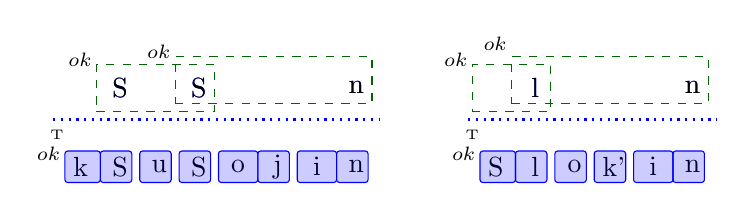
\begin{tikzpicture}
        
        \node (00) at (-0.4,0.1) {$^{ok}$};
        \node (0) at (0,0) {k};
        \node (1) at (0.5,0) {\textipa{S}};
        \node (2) at (1,0) {u};
        \node (3) at (1.5,0) {\textipa{S}};
        \node (4) at (2,0) {o};
        \node (5) at (2.5,0) {j};
        \node (6) at (3,0) {i};
        \node (7) at (3.5,0) {n};
        %tier
        \visible<3>{\node[blue] (01) at (0.5,1) {\textipa{S}};}
        \visible<4->{\node (01) at (0.5,1) {\textipa{S}};}
        \visible<5>{\node[blue] (03) at (1.5,1) {\textipa{S}};}
        \visible<6->{\node (03) at (1.5,1) {\textipa{S}};}
        \visible<9>{\node[blue] (03) at (3.5,1) {n};}
        \visible<10->{\node (03) at (3.5,1) {n};}
       
        %projection function
        \visible<2>{\filldraw [blue, rounded corners=1, fill opacity=.2,draw opacity=1] (-0.2,-0.2 ) rectangle (0.25, 0.2);}
        \visible<3>{\filldraw [blue, rounded corners=1, fill opacity=.2,draw opacity=1] (0.25,-0.2 ) rectangle (0.65, 0.2);}
        \visible<4>{\filldraw [blue, rounded corners=1, fill opacity=.2,draw opacity=1] (0.75,-0.2 ) rectangle (1.15, 0.2);}
        \visible<5>{\filldraw [blue, rounded corners=1, fill opacity=.2,draw opacity=1] (1.25,-0.2 ) rectangle (1.65, 0.2);}
        \visible<6>{\filldraw [blue, rounded corners=1, fill opacity=.2,draw opacity=1] (1.75,-0.2 ) rectangle (2.25, 0.2);}
        \visible<7>{\filldraw [blue, rounded corners=1, fill opacity=.2,draw opacity=1] (2.25,-0.2 ) rectangle (2.65, 0.2);}
        \visible<8>{\filldraw [blue, rounded corners=1, fill opacity=.2,draw opacity=1] (2.75,-0.2 ) rectangle (3.25, 0.2);}
        \visible<9>{\filldraw [blue, rounded corners=1, fill opacity=.2,draw opacity=1] (3.25,-0.2 ) rectangle (3.65, 0.2);}
        %local constraints
        \visible<10->{\draw [dashed, DarkGreen] (0.2, 0.7) -- (1.7, 0.7) -- (1.7,1.3) -- (0.2,1.3) -- (0.2, 0.7);}
        \visible<10->{\node (000) at (0,1.3) {$^{ok}$};}
        \visible<11->{\draw [dashed, DarkGreen] (1.2, 0.8) -- (3.7, 0.8) -- (3.7,1.4) -- (1.2,1.4) -- (1.2, 0.8);}
        \visible<11->{\node (000) at (1,1.4) {$^{ok}$};}
        %tier bar
        \visible<2->{\draw[dotted, thick, blue] (-0.35,0.60) to (3.8,0.60);
        \node at (-0.3,0.40) {{\tiny T}};
        }
        \begin{scope}[xshift=150pt] %string on the right
        %
        \node (00) at (-0.4,0.1) {$^{ok}$};
        \node (0) at (0,0) {\textipa{S}};
        \node (1) at (0.5,0) {l};
        \node (2) at (1,0) {o};
        \node (3) at (1.5,0) {k'};
        \node (4) at (2,0) {i };
        \node (5) at (2.5,0) {n};
        %%tier
        \visible<12>{\node[blue] (00) at (0,1) {\textesh};}
        \visible<13->{\node (00) at (0,1) {\textesh};}
        \visible<13>{\node[blue] (01) at (0.5,1) {l};}
        \visible<14->{\node (01) at (0.5,1) {l};}
        \visible<17>{\node[blue] (5) at (2.5,1) {n};}
        \visible<18->{\node (5) at (2.5,1) {n};}
        %projection function
        \visible<12>{\filldraw [blue, rounded corners=1, fill opacity=.2,draw opacity=1] (-0.2,-0.2 ) rectangle (0.25, 0.2);}
        \visible<13>{\filldraw [blue, rounded corners=1, fill opacity=.2,draw opacity=1] (0.25,-0.2 ) rectangle (0.65, 0.2);}
        \visible<14>{\filldraw [blue, rounded corners=1, fill opacity=.2,draw opacity=1] (0.75,-0.2 ) rectangle (1.15, 0.2);}
        \visible<15>{\filldraw [blue, rounded corners=1, fill opacity=.2,draw opacity=1] (1.25,-0.2 ) rectangle (1.65, 0.2);}
        \visible<16>{\filldraw [blue, rounded corners=1, fill opacity=.2,draw opacity=1] (1.75,-0.2 ) rectangle (2.25, 0.2);}
        \visible<17>{\filldraw [blue, rounded corners=1, fill opacity=.2,draw opacity=1] (2.25,-0.2 ) rectangle (2.65, 0.2);}
	%local constraints
        \visible<18->{\node (000) at (-0.5,1.3) {$^{ok}$};}
        \visible<18->{\draw [dashed, DarkGreen] (-0.3, 0.7) -- (0.7, 0.7) -- (0.7,1.3) -- (-0.3,1.3) -- (-0.3, 0.7);}
        \visible<19->{\node (000) at (0,1.5) {$^{ok}$};}
        \visible<19->{\draw [dashed, DarkGreen] (0.2, 0.8) -- (2.7, 0.8) -- (2.7,1.4) -- (0.2,1.4) -- (0.2, 0.8);}
        %tier bar
        \visible<12->{\draw[dotted, thick, blue] (-0.35,0.60) to (2.8,0.60);
        \node at (-0.3,0.40) {{\tiny T}};}
        %
        \end{scope}
        
        \end{tikzpicture}
        \end{center}

 \end{frame}  
 
 
 %==========================================%
%===================SAMALA EXAMPLE 2=======================%
%==========================================%
 \begin{frame}{Sibilant Harmony in \textsc{Samala} (2/2) }
         
         \begin{block}{Generalization (Extended)}
         	\begin{itemize}
         		\item anticipatory sibilant harmony
        			\item palatalization to avoid local restriction %against [$^*$sn,  $^*$st,  $^*$sl]
       			 \item sibilant harmony overides palatalization
         	\end{itemize}
         \end{block}
         
         \begin{exampleblock}{Grammar}
        T = \{s, \textipa{S}, n, t, l\} 
        S = \{$^*$s\textipa{S}, $^*$s\textipa{S}, $^*$sn,  $^*$st,  $^*$sl \}
        \end{exampleblock}
        
        \begin{center}
        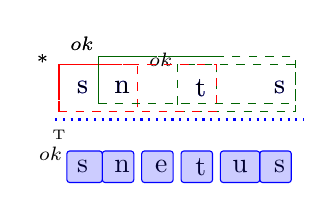
\begin{tikzpicture}%Samala 2
        \node (00) at (-0.4,0.1) {$^{ok}$};
        \node (0) at (0,0) {s};
        \node (1) at (0.5,0) {n};
        \node (2) at (1,0) {e};
        \node (3) at (1.5,0) {t};
        \node (4) at (2,0) {u };
        \node (5) at (2.5,0) {s};
        %
        %\node (00) at (-0.5,0.1) {$^{ok}$};
        %%tier
        %
        \visible<2>{\node[blue] (00) at (0,1) {s};}
        \visible<3->{\node (00) at (0,1) {s};}
        \visible<3>{\node[blue] (01) at (0.5,1) {n};}
        \visible<4->{\node (01) at (0.5,1) {n};}
        \visible<5>{\node[blue] (03) at (1.5,1) {t};}
        \visible<6->{\node (03) at (1.5,1) {t};}
        \visible<7>{\node[blue] (5) at (2.5,1) {s};}
        \visible<8->{\node (5) at (2.5,1) {s};}
        %
        %projection function
        \visible<2>{\filldraw [blue, rounded corners=1, fill opacity=.2,draw opacity=1] (-0.2,-0.2 ) rectangle (0.25, 0.2);}
        \visible<3>{\filldraw [blue, rounded corners=1, fill opacity=.2,draw opacity=1] (0.25,-0.2 ) rectangle (0.65, 0.2);}
        \visible<4>{\filldraw [blue, rounded corners=1, fill opacity=.2,draw opacity=1] (0.75,-0.2 ) rectangle (1.15, 0.2);}
        \visible<5>{\filldraw [blue, rounded corners=1, fill opacity=.2,draw opacity=1] (1.25,-0.2 ) rectangle (1.65, 0.2);}
        \visible<6>{\filldraw [blue, rounded corners=1, fill opacity=.2,draw opacity=1] (1.75,-0.2 ) rectangle (2.25, 0.2);}
        \visible<7>{\filldraw [blue, rounded corners=1, fill opacity=.2,draw opacity=1] (2.25,-0.2 ) rectangle (2.65, 0.2);}
        %local constraints
        \visible<8-10>{\node (000) at (-0.5,1.3) {$^{*}$};}
        \visible<8-10>{\draw [dashed, red] (-0.3, 0.7) -- (0.7, 0.7) -- (0.7,1.3) -- (-0.3,1.3) -- (-0.3, 0.7);}
        \visible<9-10>{\node (000) at (0,1.5) {$^{ok}$};}
        \visible<9-10>{\draw [dashed, DarkGreen] (0.2, 0.8) -- (1.7, 0.8) -- (1.7,1.4) -- (0.2,1.4) -- (0.2, 0.8);}
        \visible<10-10>{\node (000) at (1,1.3) {$^{ok}$};}
        \visible<10>{\draw [dashed, DarkGreen] (1.2, 0.7) -- (2.7, 0.7) -- (2.7,1.3) -- (1.2,1.3) -- (1.2, 0.7);}
        %%%alternative 3local
        \visible<11->{\node (000) at (-0.5,1.3) {$^{*}$};}
        \visible<11->{\draw [dashed, red] (-0.3, 0.7) -- (1.7, 0.7) -- (1.7,1.3) -- (-0.3,1.3) -- (-0.3, 0.7);}
        \visible<12->{\node (000) at (0,1.5) {$^{ok}$};}
        \visible<12->{\draw [dashed, DarkGreen] (0.2, 0.8) -- (2.7, 0.8) -- (2.7,1.4) -- (0.2,1.4) -- (0.2, 0.8);}
        %%%alternative 4local
        %\visible<13>{\node (000) at (-0.5,1.3) {$^{ok}$};}
        %\visible<13>{\draw [dashed, DarkGreen] (-0.3, 0.7) -- (2.7, 0.7) -- (2.7,1.3) -- (-0.3,1.3) -- (-0.3, 0.7);}
        %tier bar
        \visible<2->{\draw[dotted, thick, blue] (-0.35,0.60) to (2.8,0.60);
        \node at (-0.3,0.40) {{\tiny T}};}
        
        \end{tikzpicture}
        \end{center}
        \visible<13->{
        \centering
        \alert{No TSL grammar can capture this patter...}}
 \end{frame}  


 \begin{frame}{Interim Summary}

        \textbf{\textcolor{SkyBlue3!90!black}{TSL is a good fit for long distance dependencies:}}
        
        \begin{itemize}
        		\item projection of a subset of segments on a tier T;
        		\item strictly local constraints enforced on T.
        \end{itemize}
        
        \vspace{0.5cm}
        \textbf{\textcolor{SkyBlue3!90!black}{Not every attested pattern can be described this way:}}
        
        \begin{itemize}
        		\item overlapping constraints cannot work on the same tier.
       		 \item not enough information is used when projecting elements.
        \end{itemize}
        \vspace{0.5cm}
\end{frame}  
            
%%%%%%%%%%%%%%%%%%%
%==========================EXTENDING TSL ==================%
 %%%%%%%%%%%%%%%%%%+
  
            
\section[Extending the TSL Class]{Extending the TSL Class}    

 \begin{frame}{Generalizing the TSL class}
        
        TSL languages are characterized by:
        
        \begin{itemize}
        \item a \alert{1}-local projection function that projects \alert{one} tier T;
        \item strictly $k$-local constraints applied on T.
        \end{itemize} 
        
        \pause
        
        \begin{block}{Idea}
        What if ...
        \begin{enumerate}
        \item we could apply different projection functions to project \alert{multiple tiers}?
        \onslide<0>{\item the locality of the projection function was \alert{higher than 1}?}
        \end{enumerate}
        
        \end{block}
 
\end{frame}    


\begin{frame}{Multiple-Tier Strictly Local (MTSL) Languages (1/2)} %%%GOOD EXAMPLE
        \begin{exampleblock}{Sibilant Harmony in \textsc{Imdlawn Tashlhiyt} (Revisited)}
        
        Voiceless obstruents block agreement in voicing:\\
        \begin{itemize}
        \item   $T_1 = \{$\textit{\textctyogh}, s, z,\textit{\textesh}, q$\}$  $S_1= \{^*$s\textctyogh, $^*$sz, $^*$\textctyogh s,  $^*$zs, $^*$\textesh z, $^*$\textesh  \textctyogh, $^*$\textctyogh \textesh$\}$
         
        \end{itemize}
        
        \visible<9->{
        Unbounded agreement in anteriority:\\
        \begin{itemize}
        \item   $T_2 = \{$\textit{\textctyogh}, s, z,\textit{\textesh}$ \}$ $S_2= \{^*$s\textctyogh, $^*$s\textesh, $^*$\textctyogh s,$^*$\textesh s,  $^*$zs, $^*$z\textesh,  $^*$z\textctyogh, $^*$\textesh z, $^*$\textctyogh z $\}$
        \end{itemize}
        }
        \end{exampleblock}
        
        \begin{center}
        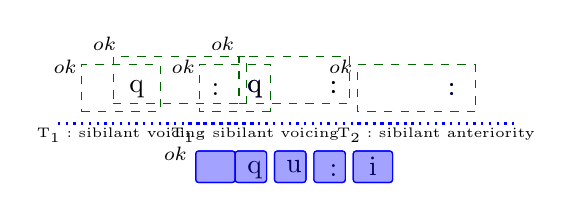
\begin{tikzpicture}%tier examples
        
        \node (000) at (-0.5,0.1) {$^{ok}$};
        \node (0) at (0,0) {\textesh};
        \node (1) at (0.5,-0.05) {q};
        \node (2) at (1,0) {u};
        \node (3) at (1.5,-0.05) { \textctyogh:};
        \node (4) at (2,0) {i};
        %tier 1 original + shifted
        \visible<2>{\node[blue] (01) at (0,1) {\textesh};}
        \visible<3-8>{\node (01) at (0,1) {\textesh};}
        \visible<3>{\node[blue] (03) at (0.5,0.98) {q};}
        \visible<4-8>{\node (03) at (0.5,0.98) {q};}
        \visible<5>{\node (03) at (1.5,1) { \textctyogh:};}
        \visible<6-8>{\node (03) at (1.5,1) { \textctyogh:};}
	%tier bar
        \visible<2-8>{
        \draw[dotted, thick, blue] (-0.35,0.55) to (2.5,0.55);
        \node at (0.5,0.40) {{\tiny T$_{1}: $ sibilant voicing}};
        }
        %local constraints
        \visible<7-8>{
        \node (00) at (-0.4,1.2) {$^{ok}$};
        \draw [dashed, DarkGreen] (0.7, 0.7) -- (-0.2, 0.7) -- (-0.2,1.3) -- (0.7,1.3) -- (0.7, 0.7);
        }
        \visible<8>{
        \node (0000) at (0.1,1.5) {$^{ok}$};
        \draw [dashed, DarkGreen] (0.3, 0.8) -- (1.7, 0.8) -- (1.7,1.4) -- (0.3,1.4) -- (0.3, 0.8);
        }
        %%%%%%%%%T1 PROJECTION FUNCTION
        \visible<2>{\filldraw [blue, rounded corners=1, fill opacity=.2,draw opacity=1] (-0.25,-0.2 ) rectangle (0.25, 0.2);}
        \visible<3>{\filldraw [blue, rounded corners=1, fill opacity=.2,draw opacity=1] (0.25,-0.2 ) rectangle (0.65, 0.2);}
        \visible<4>{\filldraw [blue, rounded corners=1, fill opacity=.2,draw opacity=1] (0.75,-0.2 ) rectangle (1.15, 0.2);}
        \visible<5>{\filldraw [blue, rounded corners=1, fill opacity=.2,draw opacity=1] (1.25,-0.2 ) rectangle (1.65, 0.2);}
        \visible<6>{\filldraw [blue, rounded corners=1, fill opacity=.2,draw opacity=1] (1.75,-0.2 ) rectangle (2.25, 0.2);}
        %%%%%%%%%%%%%%%%%%%%%%
        
        %tier 1 shifted
        \visible<9->{
        \node (0000) at (-1.4,1.5) {$^{ok}$};
        \node (00) at (-1.9,1.2) {$^{ok}$};
        \node (01) at (-1.5,1) {\textesh};
        \node (03) at (-1,0.98) {q};
        \node (05) at (0.0,0.98) {\textctyogh:};
        
        %tier 2
        \draw[dotted, thick, blue] (-2,0.55) to (0.5,0.55);
        \draw[dotted, thick, blue] (1.8,0.55) to (3.8,0.55);
        \node at (2.8,0.40) {{\tiny T$_{2}: $ sibilant anteriority }};
        \node at (-1.2,0.40) {{\tiny T$_{1}: $ sibilant voicing}};
        \draw [dashed, DarkGreen] (-1.7, 0.7) -- (-0.7, 0.7) -- (-0.7,1.3) -- (-1.7,1.3) -- (-1.7, 0.7);
        \draw [dashed, DarkGreen] (-1.3, 0.8) -- (0.4, 0.8) -- (0.4,1.4) -- (-1.3,1.4) -- (-1.3, 0.8);
        }
        
        \visible<10>{\node[blue] (02) at (2,0.98) {\textesh};}
        \visible<11->{\node (02) at (2,0.98) {\textesh};}
        
        \visible<13>{\node[blue] (06) at (3,0.98) {\textctyogh:};}
        \visible<14->{\node (06) at (3,0.98) {\textctyogh:};}
        
        \visible<15->{
        \node (000) at (1.6,1.2) {$^{ok}$};
        \draw [dashed, DarkGreen] (3.3, 0.7) -- (1.8, 0.7) -- (1.8,1.3) -- (3.3,1.3) -- (3.3, 0.7);
        }
        
        %%%%%%%%%T2 PROJECTION FUNCTION
        \visible<10>{\filldraw [blue, rounded corners=1, fill opacity=.2,draw opacity=1] (-0.25,-0.2 ) rectangle (0.25, 0.2);}
        \visible<11>{\filldraw [blue, rounded corners=1, fill opacity=.2,draw opacity=1] (0.25,-0.2 ) rectangle (0.65, 0.2);}
        \visible<12>{\filldraw [blue, rounded corners=1, fill opacity=.2,draw opacity=1] (0.75,-0.2 ) rectangle (1.15, 0.2);}
        \visible<13>{\filldraw [blue, rounded corners=1, fill opacity=.2,draw opacity=1] (1.25,-0.2 ) rectangle (1.65, 0.2);}
        \visible<14>{\filldraw [blue, rounded corners=1, fill opacity=.2,draw opacity=1] (1.75,-0.2 ) rectangle (2.25, 0.2);}
        %%%%%%%%%%%%%%%%%%%%%%
        
        \end{tikzpicture}
        \end{center}
  
\end{frame}

\begin{frame}{Multiple-Tier Strictly Local (MTSL) Languages (2/2)} % BAD EXAMPLE

        \begin{exampleblock}{Sibilant Harmony in \textsc{Imdlawn Tashlhiyt} (Revisited)}
        
        Voiceless obstruents block agreement in voicing:\\
        \begin{itemize}
        \item   $T_1 = \{$\textit{\textctyogh}, s, z,\textit{\textesh}, q$\}$  $S_1= \{^*$s\textctyogh, $^*$sz, $^*$\textctyogh s,  $^*$zs, $^*$\textesh z, $^*$\textesh  \textctyogh, $^*$\textctyogh \textesh$\}$
         
        \end{itemize}
        
        Unbounded agreement in anteriority:\\
        \begin{itemize}
        \item   $T_2 = \{$\textit{\textctyogh}, s, z,\textit{\textesh}$ \}$ $S_2= \{^*$s\textctyogh, $^*$s\textesh, $^*$\textctyogh s,$^*$\textesh s,  $^*$zs, $^*$z\textesh,  $^*$z\textctyogh, $^*$\textesh z, $^*$\textctyogh z $\}$
        \end{itemize}
        
        \end{exampleblock}

        \begin{center}
        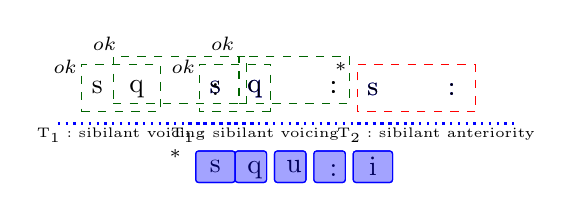
\begin{tikzpicture}%%%%MUTIPLE TIERS EXAMPLE
        
        \node (000) at (-0.5,0.1) {$^{*}$};
        \node (0) at (0,0) {s};
        \node (1) at (0.5,-0.05) {q};
        \node (2) at (1,0) {u};
        \node (3) at (1.5,-0.05) { \textctyogh:};
        \node (4) at (2,0) {i};
        %tier 1 original + shifted
        \visible<2>{\node[blue] (01) at (0,1) {s};}
        \visible<3-8>{\node (01) at (0,1) {s};}
        \visible<3>{\node[blue] (03) at (0.5,0.98) {q};}
        \visible<4-8>{\node (03) at (0.5,0.98) {q};}
        \visible<5>{\node (03) at (1.5,1) { \textctyogh:};}
        \visible<6-8>{\node (03) at (1.5,1) { \textctyogh:};}
        \visible<2-8>{
        \draw[dotted, thick, blue] (-0.35,0.55) to (2.5,0.55);
        \node at (0.5,0.40) {{\tiny T$_{1}: $ sibilant voicing}};
        }
        \visible<7-8>{
        \node (00) at (-0.4,1.2) {$^{ok}$};
        \draw [dashed, DarkGreen] (0.7, 0.7) -- (-0.2, 0.7) -- (-0.2,1.3) -- (0.7,1.3) -- (0.7, 0.7);
        }
        \visible<8>{
        \node (0000) at (0.1,1.5) {$^{ok}$};
        \draw [dashed, DarkGreen] (0.3, 0.8) -- (1.7, 0.8) -- (1.7,1.4) -- (0.3,1.4) -- (0.3, 0.8);
        }
        %%%%%%%%%T1 PROJECTION FUNCTION
        \visible<2>{\filldraw [blue, rounded corners=1, fill opacity=.2,draw opacity=1] (-0.25,-0.2 ) rectangle (0.25, 0.2);}
        \visible<3>{\filldraw [blue, rounded corners=1, fill opacity=.2,draw opacity=1] (0.25,-0.2 ) rectangle (0.65, 0.2);}
        \visible<4>{\filldraw [blue, rounded corners=1, fill opacity=.2,draw opacity=1] (0.75,-0.2 ) rectangle (1.15, 0.2);}
        \visible<5>{\filldraw [blue, rounded corners=1, fill opacity=.2,draw opacity=1] (1.25,-0.2 ) rectangle (1.65, 0.2);}
        \visible<6>{\filldraw [blue, rounded corners=1, fill opacity=.2,draw opacity=1] (1.75,-0.2 ) rectangle (2.25, 0.2);}
        %%%%%%%%%%%%%%%%%%%%%%
        %tier 2
        \visible<9->{
        \node (0000) at (-1.4,1.5) {$^{ok}$};
        \node (00) at (-1.9,1.2) {$^{ok}$};
        \node (01) at (-1.5,1) {s};
        \node (03) at (-1,0.98) {q};
        \node (05) at (0.0,0.98) {\textctyogh:};
        %tier 2
        \draw[dotted, thick, blue] (-2,0.55) to (0.5,0.55);
        \draw[dotted, thick, blue] (1.8,0.55) to (3.8,0.55);
        \node at (2.8,0.40) {{\tiny T$_{2}: $ sibilant anteriority }};
        \node at (-1.2,0.40) {{\tiny T$_{1}: $ sibilant voicing}};
        \draw [dashed, DarkGreen] (-1.7, 0.7) -- (-0.7, 0.7) -- (-0.7,1.3) -- (-1.7,1.3) -- (-1.7, 0.7);
        \draw [dashed, DarkGreen] (-1.3, 0.8) -- (0.4, 0.8) -- (0.4,1.4) -- (-1.3,1.4) -- (-1.3, 0.8);
        }
        
        \visible<10>{\node[blue] (02) at (2,0.98) {s};}
        \visible<11->{\node (02) at (2,0.98) {s};}
        
        \visible<13>{\node[blue] (06) at (3,0.98) {\textctyogh:};}
        \visible<14->{\node (06) at (3,0.98) {\textctyogh:};}
        
        \visible<15->{
        \node (000) at (1.6,1.2) {$^{*}$};
        \draw [dashed, red] (3.3, 0.7) -- (1.8, 0.7) -- (1.8,1.3) -- (3.3,1.3) -- (3.3, 0.7);
        }
        
        %%%%%%%%%T2 PROJECTION FUNCTION
        \visible<10>{\filldraw [blue, rounded corners=1, fill opacity=.2,draw opacity=1] (-0.25,-0.2 ) rectangle (0.25, 0.2);}
        \visible<11>{\filldraw [blue, rounded corners=1, fill opacity=.2,draw opacity=1] (0.25,-0.2 ) rectangle (0.65, 0.2);}
        \visible<12>{\filldraw [blue, rounded corners=1, fill opacity=.2,draw opacity=1] (0.75,-0.2 ) rectangle (1.15, 0.2);}
        \visible<13>{\filldraw [blue, rounded corners=1, fill opacity=.2,draw opacity=1] (1.25,-0.2 ) rectangle (1.65, 0.2);}
        \visible<14>{\filldraw [blue, rounded corners=1, fill opacity=.2,draw opacity=1] (1.75,-0.2 ) rectangle (2.25, 0.2);}
        %%%%%%%%%%%%%%%%%%%%%%
        
        \end{tikzpicture}
        
        \end{center}

\end{frame}

\begin{frame}{MTSL: Relations to other Classes}
        \begin{center}%new subregular region
        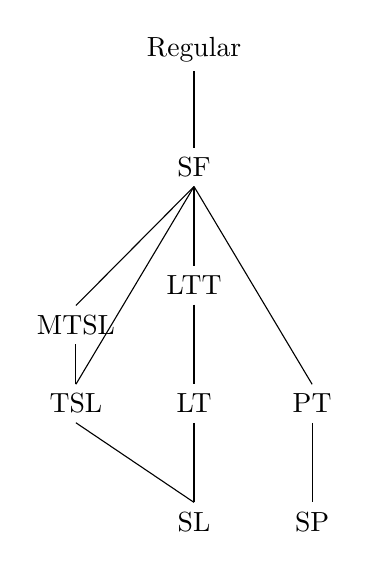
\begin{tikzpicture}[ 
            highlight/.style = { draw, rectangle, dashed }
            ]
        \node (R) at (0,10) {Regular};
        \node (SF) at (0,8.5) {SF};
        \node (LTT) at (0,7) {LTT};
        \visible<2->{\node (MTSL) at (-1.5,6.5) {MTSL};}
        \node (LT) at (0,5.5) {LT};
        \node (SL) at (0,4) {SL};
        %
        \node (PT) at (1.5,5.5) {PT};
        \node (SP) at (1.5,4) {SP};
        %
        \node (TSL) at (-1.5,5.5) {TSL};
        %
        \foreach \Source/\Target in {%
                R.south/SF.north,
                SF.south/LTT.north,
                LTT.south/LT.north,
                LT.south/SL.north,
                SF.south/PT.north,
                PT.south/SP.north,
                TSL.south/SL.north%
            }
        \draw (\Source) to (\Target);
        
        \visible<1>{  \draw ( SF.south) to (TSL.north);}
        \visible<2->{ \draw (MTSL.south) to (TSL.north);}
        \visible<3->{  \draw ( SF.south) to (MTSL.north);}
        
        \end{tikzpicture}
        \end{center}
\end{frame}

%============================GENERALIZING TSL 2 ================%
 \begin{frame}{Generalizing the TSL class (Reprise)}

        TSL languages are characterized by:
        
        \begin{itemize}
        \item a \alert{1}-local projection function that projects \alert{one} tier T;
        \item strictly $k$-local constraints applied on T.
        \end{itemize} 
        
        
        
        \begin{block}{Idea}
        
        What if ...
        \begin{enumerate}
        \item we could apply different projection functions to project \alert{multiple tiers}?
        \onslide<2->{\item the locality of the projection function was \alert{higher than 1}?}
        \end{enumerate}
        
        \end{block}
         
\end{frame}    
%====================================%====================================%
%====================================SSTSL================================%
%====================================%====================================%
\begin{frame}{Structure-Sensitive TSL (SS-TSL)} %need to pick an example

        \begin{exampleblock}{\textsc{Samala} Sibilant Harmony (Revisited)}
        
        \begin{itemize}
         \item anticipatory sibilant harmony
        \item palatalization to avoid local restrictions
        \item sibilant harmony overrides palatalization
         \end{itemize}
        \end{exampleblock}
        
        
        \begin{center}
        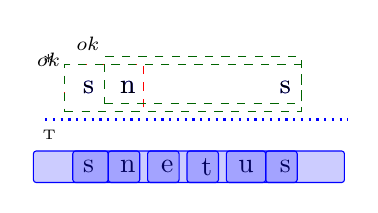
\begin{tikzpicture} %SSTSL EXAMPLE
        \visible<2->{\node (60) at (-0.5,0) {$\rtimes$};}
        \node (0) at (0,0) {s};
        \node (1) at (0.5,0) {n};
        \node (2) at (1,0) {e};
        \node (3) at (1.5,0) {t};
        \node (4) at (2,0) {u };
        \node (5) at (2.5,0) {s};
        \visible<2->{\node (6) at (3,0) {$\ltimes$};}
        %%tier
        %
        \visible<3>{\node[blue] (00) at (0,1) {s};}
        \visible<4->{\node (00) at (0,1) {s};}
        \visible<4>{\node[blue] (01) at (0.5,1) {n};}
        \visible<5->{\node (01) at (0.5,1) {n};}
        \visible<8>{\node[blue] (5) at (2.5,1) {s};}
        \visible<9->{\node (5) at (2.5,1) {s};}
        %
        %projection function
        \visible<3>{\filldraw [blue, rounded corners=1, fill opacity=.2,draw opacity=1] (-0.7,-0.2 ) rectangle (0.25, 0.2);}
        \visible<4>{\filldraw [blue, rounded corners=1, fill opacity=.2,draw opacity=1] (-0.2,-0.2 ) rectangle (0.65, 0.2);}
        \visible<5>{\filldraw [blue, rounded corners=1, fill opacity=.2,draw opacity=1] (0.25,-0.2 ) rectangle (1.15, 0.2);}
        \visible<6>{\filldraw [blue, rounded corners=1, fill opacity=.2,draw opacity=1] (0.75,-0.2 ) rectangle (1.65, 0.2);}
        \visible<7>{\filldraw [blue, rounded corners=1, fill opacity=.2,draw opacity=1] (1.25,-0.2 ) rectangle (2.25, 0.2);}
        \visible<8>{\filldraw [blue, rounded corners=1, fill opacity=.2,draw opacity=1] (1.75,-0.2 ) rectangle (2.65, 0.2);}
        \visible<9>{\filldraw [blue, rounded corners=1, fill opacity=.2,draw opacity=1] (2.25,-0.2 ) rectangle (3.25, 0.2);}
        %local constraints
        \visible<10-11>{\node (000) at (-0.5,1.3) {$^{*}$};}
        \visible<10-11>{\draw [dashed, red] (-0.3, 0.7) -- (0.7, 0.7) -- (0.7,1.3) -- (-0.3,1.3) -- (-0.3, 0.7);}
        \visible<11-11>{\node (000) at (0,1.5) {$^{ok}$};}
        \visible<11-11>{\draw [dashed, DarkGreen] (0.2, 0.8) -- (2.7, 0.8) -- (2.7,1.4) -- (0.2,1.4) -- (0.2, 0.8);}
          %local constraints   
        \visible<12->{\node (000) at (-0.5,1.3) {$^{ok}$};}
        \visible<12->{\draw [dashed, DarkGreen] (-0.3, 0.7) -- (2.7, 0.7) -- (2.7,1.3) -- (-0.3,1.3) -- (-0.3, 0.7);}
        
        %tier bar
        \visible<3->{\draw[dotted, thick, blue] (-0.55,0.60) to (3.3,0.60);
        \node at (-0.5,0.40) {{\tiny T}};}
        
        \end{tikzpicture}
        \end{center}
        
        \visible<13->{
        \begin{exampleblock}{Grammar}
        T = \{s, \textipa{S} $\wedge$ \{n, t, l\} $\triangleright$ s\} 
        S = \{$^*$s\textipa{S}, $^*$s\textipa{S}, $^*$sn($\neg$s),  $^*$st($\neg$s),   $^*$sl($\neg$s)\}
        \end{exampleblock}
        }
 \end{frame}


\begin{frame}{SS -TSL: Relations to other Classes}
\begin{center}%new subregular region
        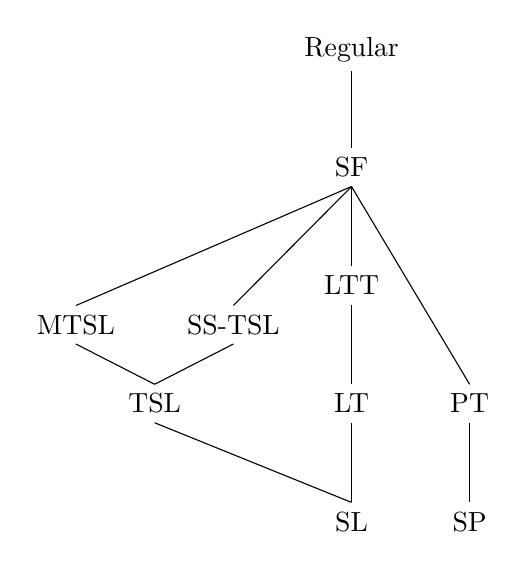
\begin{tikzpicture}[
            highlight/.style = { draw, rectangle, dashed }
            ]
        \node (R) at (0,10) {Regular};
        \node (SF) at (0,8.5) {SF};
        \node (LTT) at (0,7) {LTT};
        \node (MTSL) at (-3.5,6.5) {MTSL};
        \onslide<2->{\node (SSTSL) at (-1.5,6.5) {SS-TSL};}
        \node (LT) at (0,5.5) {LT};
        \node (SL) at (0,4) {SL};
        %
        \node (PT) at (1.5,5.5) {PT};
        \node (SP) at (1.5,4) {SP};
        %
        \node (TSL) at (-2.5,5.5) {TSL};
        %
        \foreach \Source/\Target in {%
                R.south/SF.north,
                SF.south/LTT.north,
                LTT.south/LT.north,
                LT.south/SL.north,
                SF.south/PT.north,
                PT.south/SP.north,
                SF.south/MTSL.north,
                TSL.south/SL.north,
               MTSL.south/TSL.north%
            }
        \draw (\Source) to (\Target);
        
        \onslide<2->{ \draw (SSTSL.south) to (TSL.north);}
         \onslide<3->{  \draw ( SF.south) to (SSTSL.north);}
        
        \end{tikzpicture}
        \end{center}
\end{frame}


\begin{frame}{The TSL Neighborhood: a Plethora of Combinations}
        %Expanded subregula region
        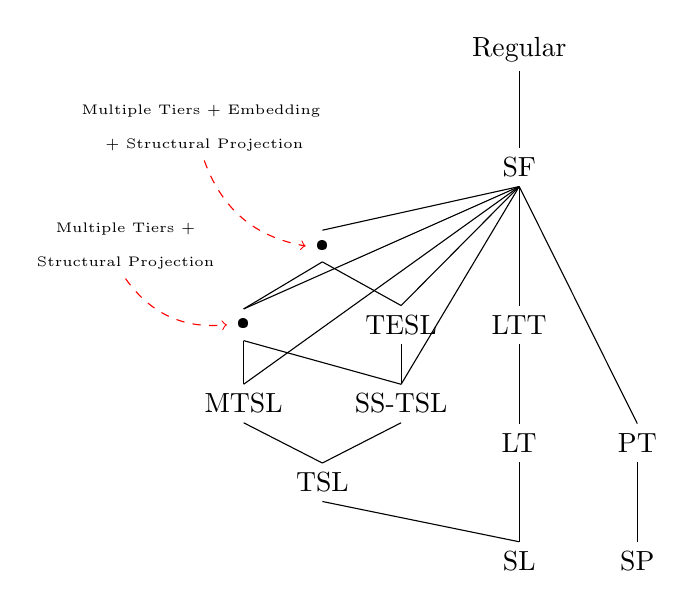
\begin{tikzpicture}[
            highlight/.style = { draw, rectangle, dashed },
            every text node part/.style={align=center}
            ]
        %\node at (0, 10.8) {\textbf{\textit{Subregular hierarchy}}};
        \node (R) at (0,10.5) {Regular};
        \node (SF) at (0,9) {SF};
        \node (LTT) at (0,7) {LTT};
        \node (LT) at (0,5.5) {LT};
        \node (SL) at (0,4) {SL};
        %
        \node (PT) at (1.5,5.5) {PT};
        \node (SP) at (1.5,4) {SP};
        %
        \visible<3->{\node(MSS) at (-3.5,7) {\textbullet};}
        \visible<4->{\node(MESS) at (-2.5,8) {\textbullet};}
        \node (MTSL) at (-3.5,6) {MTSL};
        \node (SSTSL) at (-1.5,6) {SS-TSL};
        \visible<2->{\node (TESL) at (-1.5,7) {TESL};}
        \node (TSL) at (-2.5,5) {TSL};
        %
        \foreach \Source/\Target in {%
                R.south/SF.north,
                SF.south/LTT.north,
                LTT.south/LT.north,
                LT.south/SL.north,
                SF.south/PT.north,
                PT.south/SP.north,
                TSL.south/SL.north,
               MTSL.south/TSL.north%
            }
        \draw (\Source) to (\Target);
        
        \draw (SSTSL.south) to (TSL.north);
        \visible<1>{\draw ( SF.south) to (SSTSL.north);}
        \visible<-2>{\draw ( SF.south) to (MTSL.north);}
        
        %TESL on slide 2
        \visible<2-3>{\draw ( SF.south) to (TESL.north);}
        \visible<2->{\draw ( TESL.south) to (SSTSL.north);}
        %
        %MSS on slide 3
        \visible<3>{\draw ( SF.south) to (MSS.north);}
        \visible<3->{\draw ( MSS.south) to (MTSL.north);
        \draw ( MSS.south) to (SSTSL.north);
        \node (a) at (-5,8) {\tiny{\alert{Multiple Tiers +}} \\ \tiny{\alert{Structural Projection}}};
        \draw[->, red, dashed, bend right] (a.south) to (MSS.west);
        }
        %
        %MESS on slide 4
        \visible<4->{\draw ( SF.south) to (MESS.north);
        \draw ( MESS.south) to (MSS.north);
        \draw ( MESS.south) to (TESL.north);
        \node (b) at (-4,9.5) {\tiny{\alert{Multiple Tiers +}} \tiny{\alert{Embedding }} \\ \tiny{\alert{+ Structural Projection}}};
        \draw[->, red, dashed, bend right] (b.south) to (MESS.west);
        }
        \end{tikzpicture}
        %\end{center}
\end{frame}

\section[Conclusions]{Conclusions} 

\begin{frame}{Conclusions and Future Work}
        %\begin{block}{Tracing Back our Steps}
        \textbf{\textcolor{SkyBlue3!90!black}{Tracing Back our Steps}}
        \begin{itemize}
        \item  subregular hypothesis as a strong computational theory of language complexity.  Phonology is SL + SP + TSL
        %\item current hypothesis:
        \item  but there are patterns that are unaccounted for!
        \end{itemize}
        %\end{block}
        
        \pause
        \begin{block}{In this Talk}
        \begin{itemize}
        \item TSL is not the right fit, but it seems to be close!
        \item minor changes lead to interesting new classes: MTSL, SS-TSL 
        \end{itemize}
        \end{block}
        \pause
        \begin{alertblock}{Future Work}
        \begin{itemize}
        \item further study of the TSL neighborhood 
        %\item more typological comparison is needed
        \item learnability $\rightarrow$ learning algorithms, AGL experiments ...
        \end{itemize}
        
        \end{alertblock}
 
 \end{frame}  

\begin{frame}[plain]{Selected References}
%\bibliographystyle{./acl2016}
%\nocite{Heinz2011a,Heinz2011b,HeinzRawalTanner}
%\bibliography{./acl2016.bib}

        \begin{enumerate}%weird problems with HeinzRawalTanner, fix later
        
        \item \textbf{Chandlee, Jane}. 2014. {\em Strictly Local Phonological Processes}. Ph.D. thesis, University of Delaware.
        \item \textbf{Heinz, Jeffrey}, Chetan Rawal, and Herbert~G. Tanner. 2011.Tier-based strictly local constraints in phonology. In {\em Proceedings of ACL 49th\/}, 58--64.
        \item \textbf{Heinz, Jeffrey}. 2014. Culminativity times harmony equals unbounded stress. In \textit{Word Stress: Theoretical and Typological Issues}, Chap 8.
        \item \textbf{McMullin, Kevin}. 2016.  \textit{Tier-based locality in long-distance phonotactics: learnability and typology}. Doctoral  dissertation, University of British Columbia.
        
        \end{enumerate}

\end{frame}


%%%%%%%%%%%%%%%%%%%%%APPENDIX
\unnumbered{

\begin{frame}[plain]
%
\centering
%
\huge{{\color{SkyBlue3!80!black}{Appendix}}}
%
\end{frame}

%%%%%%%%%%%%%%%
%%%%%%%%%%%%%%%FIRST LAST HARMONY %%%%%%%%%%%%%%%%%%
%%%%%%%%%%%%%%%

\begin{frame}[plain]{Structure-Sensitive TSL: Over-generation} %problems

        \begin{exampleblock}{Anticipatory Harmony in \textsc{Samala}}
        T = $\{$ s, \textesh, t\textesh$^h\}$, S= $\{ ^*$ s\textesh, $^*$\textesh s,  $^*$st\textesh$^h$,  $ ^*$t\textesh$^h\}$
        \end{exampleblock}
        
        
        
        \begin{center}
        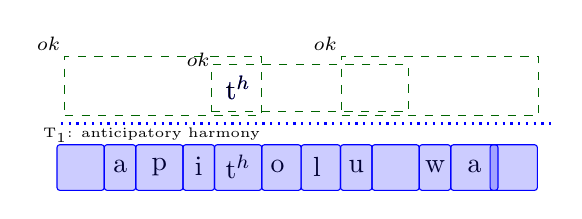
\begin{tikzpicture} %SAMALA SIBILANT HARMONY
        
        \node (0) at (0,0) {\textesh };
        \node (1) at (0.5,0) {a};
        \node (2) at (1,0) {p};
        \node (3) at (1.5,0) {i};
        \node (4) at (2,0) {};
        \node (5) at (2,0) {t\textesh$^h$};
        \node (6) at (2.5,0) {o};
        \node (7) at (3,0) {l};
        \node (8) at (3.5,0) {u};
        \node (9) at (4,0) {\textesh};
        \node (10) at (4.5,0) {w};
        \node (11) at (5,0) {a};
        \node (12) at (5.5,0) {\textesh};
        %+
        \visible<2>{\node[blue] (00) at (0,1) {\textesh };}
        \visible<3->{\node (00) at (0,1) {\textesh };}
        
        \visible<6>{\node[blue] (05) at (2,1) {t\textesh$^h$};}
        \visible<7->{\node (05) at (2,1) {t\textesh$^h$};}
        
        \visible<10>{\node[blue] (09) at (4,1) {\textesh};}
        \visible<11->{\node (09) at (4,1) {\textesh};}
        
        \visible<13>{\node[blue] (012) at (5.5,1) {\textesh};}
        \visible<14->{\node (012) at (5.5,1) {\textesh};}
        
        \visible<2->{
        \draw[dotted, thick, blue] (-0.25,0.55) to (6,0.55);
        \node at (0.9,0.40) {{\tiny T$_1$: anticipatory harmony}};
        }
        %SAMALA ISL1 projection function, keeping the porjected elements highlighted
        \visible<2,14->{\filldraw [blue, rounded corners=1, fill opacity=.2,draw opacity=1] (-0.3,-0.3 ) rectangle (0.3, 0.28);}
        %
        \visible<3>{\filldraw [blue, rounded corners=1, fill opacity=.2,draw opacity=1] (0.3,-0.3 ) rectangle (0.7, 0.28);}%
        \visible<4>{\filldraw [blue, rounded corners=1, fill opacity=.2,draw opacity=1] (0.7,-0.3 ) rectangle (1.3, 0.28);}%
        \visible<5>{\filldraw [blue, rounded corners=1, fill opacity=.2,draw opacity=1] (1.3,-0.3 ) rectangle (1.7, 0.28);}%
        %
        \visible<6,14->{\filldraw [blue, rounded corners=1, fill opacity=.2,draw opacity=1] (1.7,-0.3 ) rectangle (2.3, 0.28);}
        %
        \visible<7>{\filldraw [blue, rounded corners=1, fill opacity=.2,draw opacity=1] (2.3,-0.3 ) rectangle (2.8, 0.28);}%
        \visible<8>{\filldraw [blue, rounded corners=1, fill opacity=.2,draw opacity=1] (2.8,-0.3 ) rectangle (3.3, 0.28);}%
        \visible<9>{\filldraw [blue, rounded corners=1, fill opacity=.2,draw opacity=1] (3.3,-0.3 ) rectangle (3.7, 0.28);}%
        %
        \visible<10,14->{\filldraw [blue, rounded corners=1, fill opacity=.2,draw opacity=1] (3.7,-0.3 ) rectangle (4.3, 0.28);}
        %
        \visible<11>{\filldraw [blue, rounded corners=1, fill opacity=.2,draw opacity=1] (4.3,-0.3 ) rectangle (4.7, 0.28);}%
        \visible<12>{\filldraw [blue, rounded corners=1, fill opacity=.2,draw opacity=1] (4.7,-0.3 ) rectangle (5.3, 0.28);}%
        %
        \visible<13,14->{\filldraw [blue, rounded corners=1, fill opacity=.2,draw opacity=1] (5.2,-0.3 ) rectangle (5.8, 0.28);}
        
        \visible<14->{\draw [dashed, DarkGreen] (-0.2, 0.65) -- (2.3, 0.65) -- (2.3,1.4) -- (-0.2,1.4) -- (-0.2, 0.65);
        \node (000) at (-0.4,1.5) {$^{ok}$};
        }
        
        \visible<15->{
        \begin{scope}[xshift=53pt]
        \draw [dashed, DarkGreen] (-0.2, 0.7) -- (2.3, 0.7) -- (2.3,1.3) -- (-0.2,1.3) -- (-0.2, 0.7);
        \end{scope}
        \node (0000) at (1.5,1.3) {$^{ok}$};
        }
        %
        \visible<16->{
        \begin{scope}[xshift=100pt]
        \node (000) at (-0.4,1.5) {$^{ok}$};
        \draw [dashed, DarkGreen] (-0.2, 0.65) -- (2.3, 0.65) -- (2.3,1.4) -- (-0.2,1.4) -- (-0.2, 0.65);
        \end{scope}
        }
        
        \end{tikzpicture}
        \end{center}
        
        
        \visible<17->{
        \begin{exampleblock}{First/Last Harmony in \textsc{Pseudo-Samala}}
        T = $\{ \sigma$: $\sigma \in \{$s, \textesh, t\textesh$^h \}$ $\wedge (\rtimes \sigma \vee \sigma \ltimes) \}$ S= $\{ ^*$s\textesh, $^*$\textesh s,  $^*$st\textesh$^h$,  $^*$t\textesh$^h$ s$\}$
        
        \end{exampleblock}
        }
        
        \begin{center}
        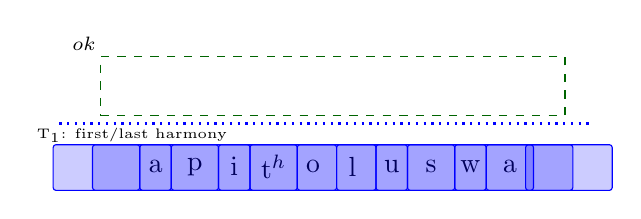
\begin{tikzpicture}%PSEUDO SAMALA FIRST LAST HARMONY, 
        
        \begin{scope}%[yshift=-100pt]
        
        \visible<17->{
        \node (0) at (0,0) {\textesh };
        \node (1) at (0.5,0) {a};
        \node (2) at (1,0) {p};
        \node (3) at (1.5,0) {i};
        \node (4) at (2,0) {};
        \node (5) at (2,0) {t\textesh$^h$};
        \node (6) at (2.5,0) {o};
        \node (7) at (3,0) {l};
        \node (8) at (3.5,0) {u};
        \node (9) at (4,0) {s};
        \node (10) at (4.5,0) {w};
        \node (11) at (5,0) {a};
        \node (12) at (5.5,0) {\textesh};
        }
        
        \visible<18->{\node (000) at (-0.5,0) {$\rtimes$};
        \node (0000) at (6,0) {$\ltimes$};
        }
        %
        \visible<19,32->{\filldraw [blue, rounded corners=1, fill opacity=.2,draw opacity=1] (-0.8,-0.3 ) rectangle (0.3, 0.28);}
        %%%%%
        %%
        \visible<20>{\filldraw [blue, rounded corners=1, fill opacity=.2,draw opacity=1](-0.3,-0.3 )rectangle (0.7, 0.28);}%
        \visible<21>{\filldraw [blue, rounded corners=1, fill opacity=.2,draw opacity=1] (0.3,-0.3 ) rectangle (1.3, 0.28);}%
        \visible<22>{\filldraw [blue, rounded corners=1, fill opacity=.2,draw opacity=1] (0.7,-0.3 ) rectangle (1.7, 0.28);}%
        %%
        \visible<23>{\filldraw [blue, rounded corners=1, fill opacity=.2,draw opacity=1](1.3,-0.3 ) rectangle  (2.3, 0.28);}
        \visible<24>{\filldraw [blue, rounded corners=1, fill opacity=.2,draw opacity=1] (1.7,-0.3 )  rectangle ((2.8, 0.28);}
        \visible<25>{\filldraw [blue, rounded corners=1, fill opacity=.2,draw opacity=1] (2.3,-0.3 ) rectangle (3.3, 0.28);}%ol
        \visible<26>{\filldraw [blue, rounded corners=1, fill opacity=.2,draw opacity=1] (2.8,-0.3 ) rectangle (3.7, 0.28);}%lu
        %%
        \visible<27>{\filldraw [blue, rounded corners=1, fill opacity=.2,draw opacity=1] (3.3,-0.3 ) rectangle (4.3, 0.28);}%us
        \visible<28>{\filldraw [blue, rounded corners=1, fill opacity=.2,draw opacity=1] (3.7,-0.3 )  rectangle  (4.7, 0.28);}%sw
        \visible<29>{\filldraw [blue, rounded corners=1, fill opacity=.2,draw opacity=1] (4.3,-0.3 ) rectangle (5.3, 0.28);}
        \visible<30>{\filldraw [blue, rounded corners=1, fill opacity=.2,draw opacity=1] (4.7,-0.3 ) rectangle (5.8, 0.28);}
        
        \visible<31->{\filldraw [blue, rounded corners=1, fill opacity=.2,draw opacity=1] (5.2,-0.3 )rectangle (6.3, 0.28);}
        
        \visible<19>{\node[blue] (00) at (0,1) {\textesh };}
        \visible<20->{\node (00) at (0,1) {\textesh };}
        
        \visible<31>{\node[blue] (012) at (5.5,1) {\textesh};}
        \visible<32->{\node (012) at (5.5,1) {\textesh};}
           
        \visible<19->{
        \draw[dotted, thick, blue] (-0.72,0.55) to (6,0.55);
        \node at (0.2,0.40) {{\tiny T$_1$: first/last harmony}};
        }
        
        \visible<32->{\draw [dashed, DarkGreen] (-0.2, 0.65) -- (5.7, 0.65) -- (5.7,1.4) -- (-0.2,1.4) -- (-0.2, 0.65);
        \node (0000) at (-0.4,1.5) {$^{ok}$};
        }
        \end{scope}
        
        \end{tikzpicture}
        \end{center}
\end{frame}


\begin{frame}[plain]{Closure Properties of Subregular Classes}

        \begin{table}[]
        \centering
        \label{my-label}
        \begin{tabular}{ccccccc}
                   & SL         & TSL        & MTSL       & SS-TSL     & SF         & Reg      \\
        $\cup$     & $\times$ & $\times$ & $\times$ & $\times$ & \checkmark  & \checkmark\\
        $\cap$     & \checkmark  & $\times$ & \checkmark  &$\times$ & \checkmark  & \checkmark\\
        Relabeling &$\times$ &$\times$ & $\times$ &$\times$ & $\times$ & \checkmark\\
        Complement &$\times$ &$\times$ &$\times$ & $\times$ & \checkmark  & \checkmark
        \end{tabular}
        \end{table}

\end{frame}

}


  \end{document}            
            
